\documentclass[11pt, oneside]{article}   	% use "amsart" instead of "article" for AMSLaTeX format
\usepackage{geometry}                		% See geometry.pdf to learn the layout options. There are lots.
\geometry{letterpaper}                   		% ... or a4paper or a5paper or ... 
%\geometry{landscape}                		% Activate for rotated page geometry
%\usepackage[parfill]{parskip}    		% Activate to begin paragraphs with an empty line rather than an indent
\usepackage{graphicx}				% Use pdf, png, jpg, or eps§ with pdflatex; use eps in DVI mode
								% TeX will automatically convert eps --> pdf in pdflatex		
\usepackage{amssymb}

%SetFonts

%SetFonts

\geometry{margin=.5in}
\title{Model Documentation}
\author{}
%\date{}							% Activate to display a given date or no date

\begin{document}
\maketitle

\section{Overview}
\section{Background}
\section{Theory}

\subsubsection{Model Specification}
%A neural mass model based on hippocampal model developed by Wendling et al. was extended to simulate the dynamics of the CA1 to CA3 pathway in the rat hippocampus \cite{Wendling2002}.  Structurally, this model is composed of two masses representing the CA3 and CA1 regions of the hippocampus, each containing three neuronal populations: excitatory, fast inhibitory and slow inhibitory. The excitatory population of the CA3 neurons project to the excitatory populations of the CA1 model (Schaffer collaterals), and conversely a subset of fast inhibitory population feeds back to the excitatory subset of the CA3 population (Figure \ref{fig:fig_1})\cite{Sik1994}. Each neuron type is represented by a second order linear transfer function composed of an impulse function $h_e(t)$, $h_{if}(t)$, and $h_{is}(t)$ and an asymmetric sigmoid function that transforms the average synaptic pulse density to an average post synaptic membrane potential. The impulse response functions are defined as  $h_{e}(t) = Aae^{-at}$, $h_{if}(t) = Bbe^{-bt}$ and $h_{is}(t) = Gge^{-gt}$, where $A$, $B$, $G$and  are the synaptic gains, and $1/a$, $1/b$, and $1/g$ are the synaptic delays. These transfer function leads to the formulation of a set of second order ordinary differential equations for each population of the form: 
% 
%\begin{equation}
%\ddot{y}_i=W_i w_i z_i-2w_i\dot{y}_i-w_i^2 y_i
%\end{equation}
%\begin{equation}
%z_i=S(v_i )=\frac{2e}{1+e^{-rv_i } }-e_0
%\end{equation}
%\begin{equation}
%v_i=C_{ij} y_j+u_i(t)
%\end{equation}
%
%$C_1,C_2,\dots,C_7$, detailed in \cite{Wendling2002} along with two additional connectivity parameters $C_{schaffer}$ and $C_{feedback}$ the describe the excitatory projections from CA3 to CA1 and the inhibitory projections from CA1 to CA3. This set of 22 differential equations was solved using a first order Euler method with a 2000Hz timestep. The inputs to the model are Gaussian noise signals applied to the excitatory interneurons of the CA3 and CA1 regions independently. The two output of the model are the individual sums of the average postsynaptic potentials for the excitatory, slow inhibitory and fast inhibitory neuronal populations in CA3 and CA3.

\section{Architecture}
\subsection{Motivation}
\subsubsection{Modular Software Architecture}
While the CA3\_CA1 model is still in a proof-of-concept stage it will serve as the foundation for a larger project to generate models based on \textit{in vivo} experiments and prototype neuromodulation systems. To facilitate this project it is necessary to have a robust computational platform to integrate these steps. This is accomplished through a modular system architecture that will allow for the different components of the platform (mathematical model, optimization program, interface, etc) to be developed in parallel and extended as the overall application matures. 

The other advantage for a modular architecture is the ability to develop a set of unit tests that can verify new changes do not have undetected effects by regressing against ground truths and previous versions. Finally, when these bugs are detected, the clear delineation between software components will decrease the amount of time necessary to fix. 

\subsubsection{Dynamic Specification of Model Structure}
While the overall application maintains a modular architecture, the computational core of model needs to also be dynamic so that models of different structure and parameterization can be configured on the fly. The most immediate focus is the septohippocampal model which acts as the primary \textit{in vivo} arm of the project, and can use different implants - electrodes or fiber optic ferrules, different optogenetic constructs, viral promoters, and different LED wavelengths.

In addition to the varied configurations of the septohippocampal model, there are several additional datasets from other studies becoming available. However, these data sets use different signal modalities in the case of data from patients receiving deep brain stimulation for treatment resistant depression, and can have structural properties that vary between patients in the DARPA Restoring Active Memory (RAM) trial. 

\subsubsection{Validation and Refinement}
By using a robust software architecture that allows for flexible and agile development it will increase the rate of adaptation with the Emory neuroengineering community. This will allow the scientific theory underlying the model to be validated in a variety of contexts and experimental environments. Furthermore, the different operating systems used among the different labs will encourage cross-platform development and testing from the ground up rather than porting after the code base is more developed. Finally, building a system that can generalize to the needs of different users will serve to further test and refine the application.

\subsection{Design}
\begin{figure}[h!]
	\centering
	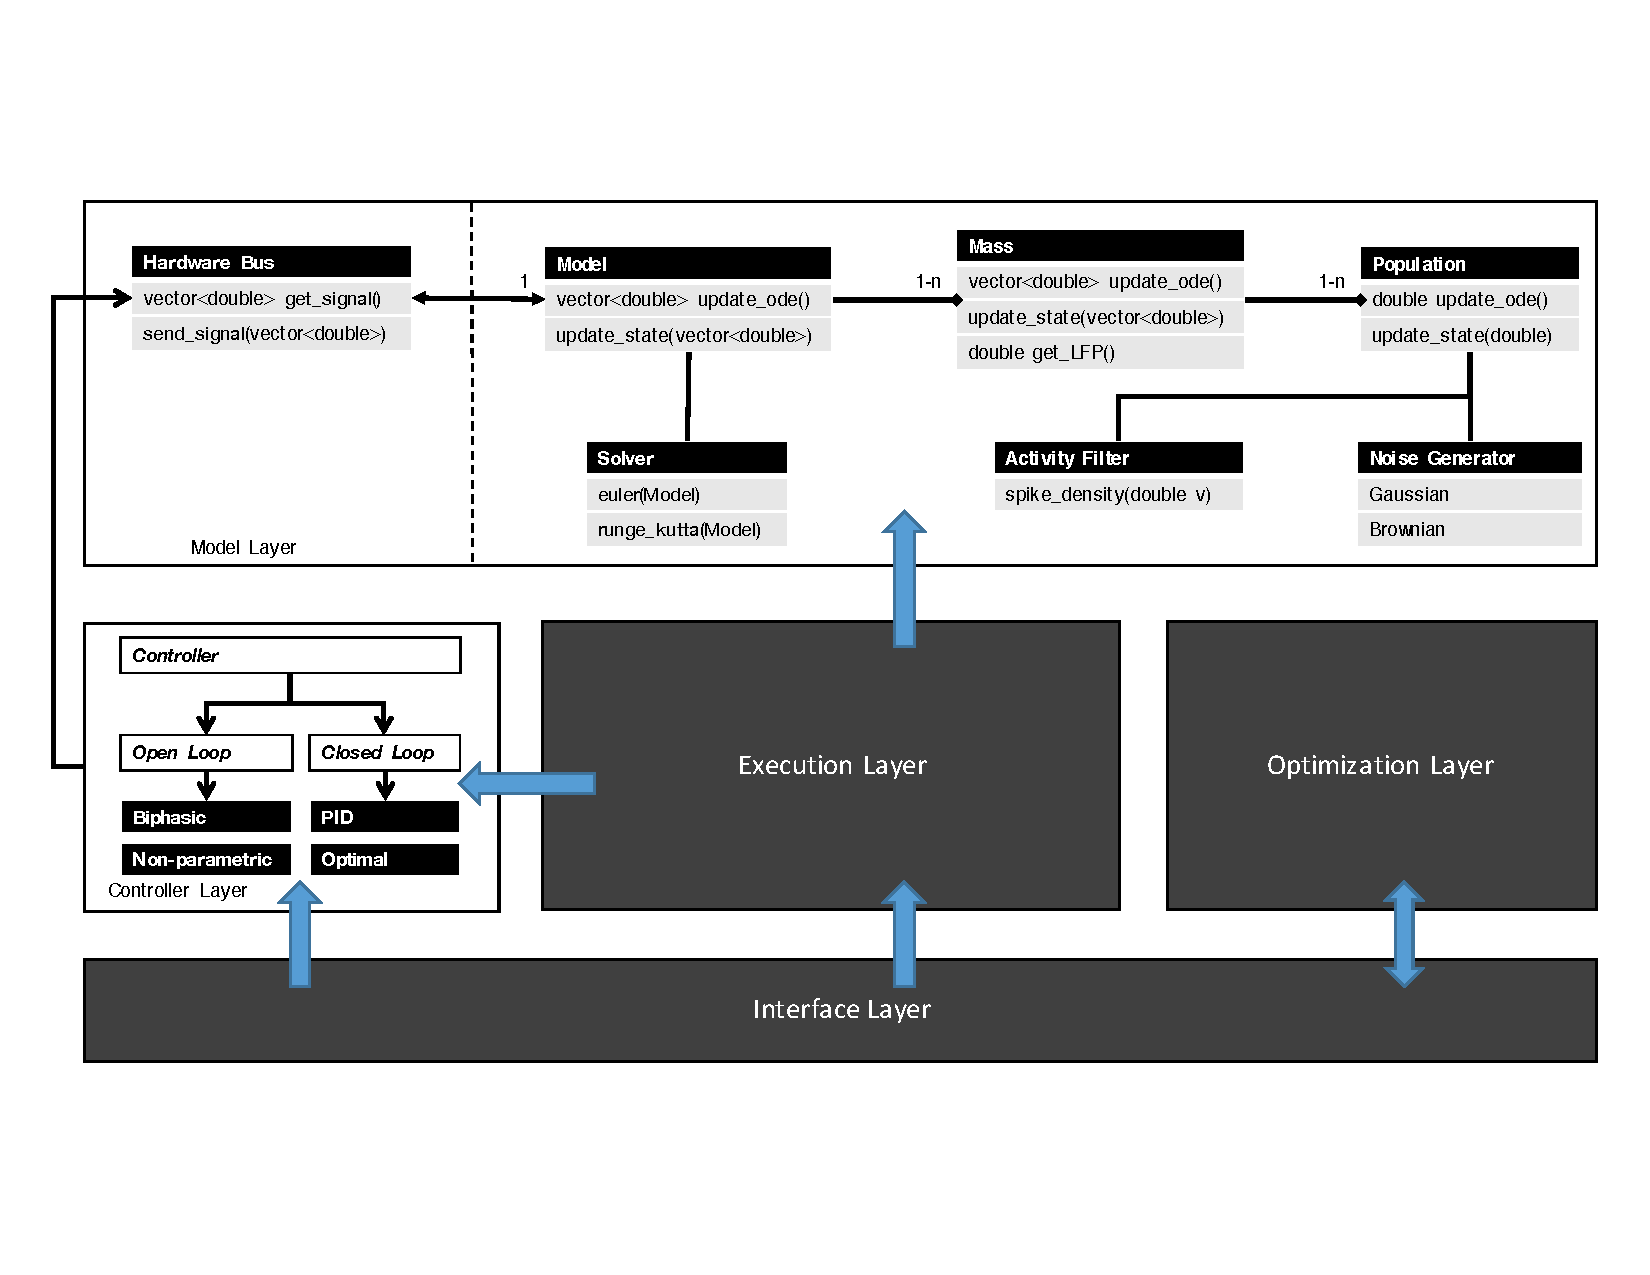
\includegraphics[width=\textwidth,height=\textheight,keepaspectratio]{Software_Architecture.pdf}
	\caption{Software Architecture Diagram}
\end{figure}

\section{Operation}
\section{API}



\end{document}  